% ============================================================
% Question Bank: ch06-01 Understanding and Using Scale Drawings
% Topic Title: Understanding and Using Scale Drawings
% CCSS: 7.G.A.1
% Questions: 27 (15 MC + 6 SA + 6 Graphical)
% ============================================================

% --- Multiple Choice Questions (15) ---

\begin{practiceQuestion}{6-1-q01}{mc}
\begin{questionText}
A trail map uses the scale $1$ cm $= 15$ km. Two campsites are $7$ cm apart on the map. What is the actual distance between the campsites?
\end{questionText}
\choiceA{$22$ km}
\choiceB{$75$ km}
\choiceC{$105$ km}
\choiceD{$115$ km}
\correctAnswer{C}
\explanation{Multiply the map distance by the scale factor: $7 \times 15 = 105$ km. Each centimeter on the map represents $15$ km in real life.}
\end{practiceQuestion}

\begin{practiceQuestion}{6-1-q02}{mc}
\begin{questionText}
An architect's blueprint uses the scale $1$ in $= 5$ ft. A kitchen is $3.6$ in wide on the blueprint. What is the actual width of the kitchen?
\end{questionText}
\choiceA{$15$ ft}
\choiceB{$18$ ft}
\choiceC{$20$ ft}
\choiceD{$36$ ft}
\correctAnswer{B}
\explanation{Multiply the drawing length by the scale factor: $3.6 \times 5 = 18$ ft.}
\end{practiceQuestion}

\begin{practiceQuestion}{6-1-q03}{mc}
\begin{questionText}
A model spacecraft uses a scale of $1:48$. The model is $15$ inches long. What is the actual length of the spacecraft?
\end{questionText}
\choiceA{$63$ inches}
\choiceB{$480$ inches}
\choiceC{$720$ inches}
\choiceD{$3.2$ inches}
\correctAnswer{C}
\explanation{Multiply the model length by the scale factor: $15 \times 48 = 720$ inches.}
\end{practiceQuestion}

\begin{practiceQuestion}{6-1-q04}{mc}
\begin{questionText}
On a road map, $4$ cm represents $60$ km. What distance does $1$ cm represent?
\end{questionText}
\choiceA{$4$ km}
\choiceB{$15$ km}
\choiceC{$24$ km}
\choiceD{$56$ km}
\correctAnswer{B}
\explanation{Find the unit rate: $60 \div 4 = 15$ km per cm. Each centimeter on the map represents $15$ km.}
\end{practiceQuestion}

\begin{practiceQuestion}{6-1-q05}{mc}
\begin{questionText}
A floor plan uses $1$ cm $= 3$ m. A bathroom is $2$ cm by $2.5$ cm on the plan. What is the actual area of the bathroom?
\end{questionText}
\choiceA{$5$ m$^2$}
\choiceB{$15$ m$^2$}
\choiceC{$30$ m$^2$}
\choiceD{$45$ m$^2$}
\correctAnswer{D}
\explanation{Actual dimensions: $2 \times 3 = 6$ m and $2.5 \times 3 = 7.5$ m. Actual area: $6 \times 7.5 = 45$ m$^2$.}
\end{practiceQuestion}

\begin{practiceQuestion}{6-1-q06}{mc}
\begin{questionText}
If a scale factor is $4$, by what factor does the area of the actual figure compare to the area of the scale drawing?
\end{questionText}
\choiceA{$4$ times as large}
\choiceB{$8$ times as large}
\choiceC{$16$ times as large}
\choiceD{$64$ times as large}
\correctAnswer{C}
\explanation{When lengths scale by $k$, areas scale by $k^2$. Here $k = 4$, so area scales by $4^2 = 16$.}
\end{practiceQuestion}

\begin{practiceQuestion}{6-1-q07}{mc}
\begin{questionText}
A soccer field is $100$ m long. On a scale drawing, it appears as $5$ cm. What scale does the drawing use?
\end{questionText}
\choiceA{$1$ cm $= 10$ m}
\choiceB{$1$ cm $= 15$ m}
\choiceC{$1$ cm $= 20$ m}
\choiceD{$1$ cm $= 25$ m}
\correctAnswer{C}
\explanation{Divide the actual length by the drawing length: $100 \div 5 = 20$. The scale is $1$ cm $= 20$ m.}
\end{practiceQuestion}

\begin{practiceQuestion}{6-1-q08}{mc}
\begin{questionText}
A skyscraper is $960$ ft tall. A scale model uses a scale of $1$ in $= 16$ ft. How tall is the model?
\end{questionText}
\choiceA{$48$ in}
\choiceB{$60$ in}
\choiceC{$64$ in}
\choiceD{$96$ in}
\correctAnswer{B}
\explanation{Divide the actual height by the scale factor: $960 \div 16 = 60$ inches.}
\end{practiceQuestion}

\begin{practiceQuestion}{6-1-q09}{mc}
\begin{questionText}
A dollhouse uses a scale of $1:12$. A real dining table is $60$ inches long. How long is the dollhouse table?
\end{questionText}
\choiceA{$3$ inches}
\choiceB{$5$ inches}
\choiceC{$12$ inches}
\choiceD{$48$ inches}
\correctAnswer{B}
\explanation{Divide the actual length by the scale factor: $60 \div 12 = 5$ inches.}
\end{practiceQuestion}

\begin{practiceQuestion}{6-1-q10}{mc}
\begin{questionText}
A triangular park is drawn on a map with $1$ cm $= 10$ m. The triangle's base is $3$ cm and its height is $4$ cm on the map. What is the actual area of the park?
\end{questionText}
\choiceA{$6$ m$^2$}
\choiceB{$60$ m$^2$}
\choiceC{$600$ m$^2$}
\choiceD{$1{,}200$ m$^2$}
\correctAnswer{C}
\explanation{Actual base: $3 \times 10 = 30$ m, actual height: $4 \times 10 = 40$ m. Area $= \frac{1}{2} \times 30 \times 40 = 600$ m$^2$.}
\end{practiceQuestion}

\begin{practiceQuestion}{6-1-q11}{mc}
\begin{questionText}
A highway map shows $1$ cm $= 35$ km. Natasha measures the distance between two exits as $2.4$ cm. What is the actual distance?
\end{questionText}
\choiceA{$70$ km}
\choiceB{$84$ km}
\choiceC{$37.4$ km}
\choiceD{$14.6$ km}
\correctAnswer{B}
\explanation{Multiply the map distance by the scale factor: $2.4 \times 35 = 84$ km.}
\end{practiceQuestion}

\begin{practiceQuestion}{6-1-q12}{mc}
\begin{questionText}
A square room is $4$ cm on each side on a blueprint with scale $1$ cm $= 6$ ft. What is the actual area of the room?
\end{questionText}
\choiceA{$96$ ft$^2$}
\choiceB{$144$ ft$^2$}
\choiceC{$576$ ft$^2$}
\choiceD{$24$ ft$^2$}
\correctAnswer{C}
\explanation{Actual side: $4 \times 6 = 24$ ft. Actual area: $24 \times 24 = 576$ ft$^2$.}
\end{practiceQuestion}

\begin{practiceQuestion}{6-1-q13}{mc}
\begin{questionText}
Which statement about scale drawings is FALSE?
\end{questionText}
\choiceA{Angles in the drawing are the same as the actual angles}
\choiceB{If the scale factor is $k$, areas scale by $k^2$}
\choiceC{All lengths are multiplied by the same scale factor}
\choiceD{If the scale factor doubles, the area also doubles}
\correctAnswer{D}
\explanation{If the scale factor doubles, lengths double, but areas scale by the square of the length change. Doubling the scale factor quadruples the area, so statement D is false.}
\end{practiceQuestion}

\begin{practiceQuestion}{6-1-q14}{mc}
\begin{questionText}
A lake is $300$ m wide. On a map, it is shown as $12$ cm wide. What is the map's scale factor?
\end{questionText}
\choiceA{$1$ cm $= 20$ m}
\choiceB{$1$ cm $= 25$ m}
\choiceC{$1$ cm $= 30$ m}
\choiceD{$1$ cm $= 36$ m}
\correctAnswer{B}
\explanation{Divide the actual width by the drawing width: $300 \div 12 = 25$. The scale is $1$ cm $= 25$ m.}
\end{practiceQuestion}

\begin{practiceQuestion}{6-1-q15}{mc}
\begin{questionText}
A museum exhibit features a scale model of a whale. The real whale is $90$ ft long. The model is $6$ ft long. What is the scale of the model?
\end{questionText}
\choiceA{$1:6$}
\choiceB{$1:9$}
\choiceC{$1:15$}
\choiceD{$1:90$}
\correctAnswer{C}
\explanation{Scale $= \frac{\text{model}}{\text{actual}} = \frac{6}{90} = \frac{1}{15}$. The model uses scale $1:15$.}
\end{practiceQuestion}

% --- Short Answer Questions (6) ---

\begin{practiceQuestion}{6-1-q16}{sa}
\begin{questionText}
A city map uses $1$ cm $= 12$ km. Two hospitals are $8.5$ cm apart on the map. What is the actual distance between the hospitals?
\end{questionText}
\correctAnswer{$102$ km}
\explanation{Multiply the map distance by the scale factor: $8.5 \times 12 = 102$ km.}
\end{practiceQuestion}

\begin{practiceQuestion}{6-1-q17}{sa}
\begin{questionText}
A blueprint uses $1$ in $= 7$ ft. A patio is $56$ ft long in real life. How long is the patio on the blueprint?
\end{questionText}
\correctAnswer{$8$ in}
\explanation{Divide the actual length by the scale factor: $56 \div 7 = 8$ in.}
\end{practiceQuestion}

\begin{practiceQuestion}{6-1-q18}{sa}
\begin{questionText}
A rectangular playground is $4$ cm by $6$ cm on a map with scale $1$ cm $= 15$ m. What is the actual area of the playground?
\end{questionText}
\correctAnswer{$5{,}400$ m$^2$}
\explanation{Actual dimensions: $4 \times 15 = 60$ m and $6 \times 15 = 90$ m. Actual area: $60 \times 90 = 5{,}400$ m$^2$.}
\end{practiceQuestion}

\begin{practiceQuestion}{6-1-q19}{sa}
\begin{questionText}
A model train has a scale of $1:87$. If the model engine is $3$ inches long, how long is the actual engine in inches?
\end{questionText}
\correctAnswer{$261$ inches}
\explanation{Multiply by the scale factor: $3 \times 87 = 261$ inches.}
\end{practiceQuestion}

\begin{practiceQuestion}{6-1-q20}{sa}
\begin{questionText}
On a scale drawing, a warehouse is $5$ cm by $8$ cm. The scale is $1$ cm $= 9$ m. What is the actual perimeter of the warehouse?
\end{questionText}
\correctAnswer{$234$ m}
\explanation{Actual dimensions: $5 \times 9 = 45$ m and $8 \times 9 = 72$ m. Perimeter: $2(45 + 72) = 2(117) = 234$ m.}
\end{practiceQuestion}

\begin{practiceQuestion}{6-1-q21}{sa}
\begin{questionText}
A drawing uses a scale factor of $6$. A rectangle on the drawing has an area of $10$ cm$^2$. What is the actual area?
\end{questionText}
\correctAnswer{$360$ cm$^2$}
\explanation{Area scales by $k^2 = 6^2 = 36$. Actual area: $10 \times 36 = 360$ cm$^2$.}
\end{practiceQuestion}

% --- Graphical MC Questions (3) ---

\begin{practiceQuestion}{6-1-q22}{gmc}
\begin{questionText}
The scale drawing below shows a rectangular office. The scale is $1$ cm $= 4$ m. What is the actual area of the office?

\begin{center}
\begin{tikzpicture}[scale=0.7]
  \draw[thick,fill=funBlue!10] (0,0) rectangle (5,3);
  \draw[<->] (0,-0.4) -- (5,-0.4);
  \node[below] at (2.5,-0.4) {$5$ cm};
  \draw[<->] (5.4,0) -- (5.4,3);
  \node[right] at (5.4,1.5) {$3$ cm};
  \node at (2.5,1.5) {\small Office};
\end{tikzpicture}
\end{center}
\end{questionText}
\choiceA{$15$ m$^2$}
\choiceB{$60$ m$^2$}
\choiceC{$192$ m$^2$}
\choiceD{$240$ m$^2$}
\correctAnswer{D}
\explanation{Actual dimensions: $5 \times 4 = 20$ m and $3 \times 4 = 12$ m. Actual area: $20 \times 12 = 240$ m$^2$.}
\end{practiceQuestion}

\begin{practiceQuestion}{6-1-q23}{gmc}
\begin{questionText}
A map uses $1$ cm $= 10$ km. The route between three towns is shown below. What is the total actual distance from Town A to Town B to Town C?

\begin{center}
\begin{tikzpicture}[scale=0.9]
  \node[circle,draw,fill=funBlue!30,inner sep=2pt] (A) at (0,0) {\small A};
  \node[circle,draw,fill=funBlue!30,inner sep=2pt] (B) at (4,0) {\small B};
  \node[circle,draw,fill=funBlue!30,inner sep=2pt] (C) at (4,3) {\small C};
  \draw[thick] (A) -- (B) node[midway,below] {$4$ cm};
  \draw[thick] (B) -- (C) node[midway,right] {$3$ cm};
\end{tikzpicture}
\end{center}
\end{questionText}
\choiceA{$7$ km}
\choiceB{$50$ km}
\choiceC{$70$ km}
\choiceD{$120$ km}
\correctAnswer{C}
\explanation{Total map distance: $4 + 3 = 7$ cm. Actual distance: $7 \times 10 = 70$ km.}
\end{practiceQuestion}

\begin{practiceQuestion}{6-1-q24}{gmc}
\begin{questionText}
The scale drawing below shows an L-shaped room. The scale is $1$ cm $= 2$ m. What is the actual area of the room?

\begin{center}
\begin{tikzpicture}[scale=0.6]
  \draw[thick,fill=funBlue!10] (0,0) -- (6,0) -- (6,2) -- (3,2) -- (3,4) -- (0,4) -- cycle;
  \draw[<->] (0,-0.4) -- (6,-0.4);
  \node[below] at (3,-0.4) {$6$ cm};
  \draw[<->] (-0.4,0) -- (-0.4,4);
  \node[left] at (-0.4,2) {$4$ cm};
  \draw[<->] (3,2.3) -- (6,2.3);
  \node[above] at (4.5,2.3) {$3$ cm};
  \draw[<->] (6.4,0) -- (6.4,2);
  \node[right] at (6.4,1) {$2$ cm};
\end{tikzpicture}
\end{center}
\end{questionText}
\choiceA{$18$ m$^2$}
\choiceB{$60$ m$^2$}
\choiceC{$72$ m$^2$}
\choiceD{$96$ m$^2$}
\correctAnswer{C}
\explanation{Drawing area: top part is $3 \times 2 = 6$ cm$^2$, bottom part is $6 \times 2 = 12$ cm$^2$, total $= 18$ cm$^2$. Area scales by $2^2 = 4$. Actual area: $18 \times 4 = 72$ m$^2$.}
\end{practiceQuestion}

% --- Graphical SA Questions (3) ---

\begin{practiceQuestion}{6-1-q25}{gsa}
\begin{questionText}
The scale drawing below shows a triangular garden. The scale is $1$ cm $= 5$ m. Find the actual area of the garden.

\begin{center}
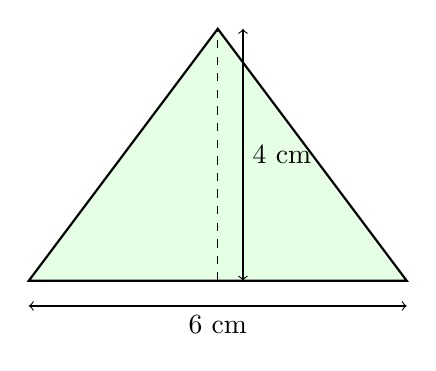
\begin{tikzpicture}[scale=0.8]
  \draw[thick,fill=green!10] (0,0) -- (6,0) -- (3,4) -- cycle;
  \draw[<->] (0,-0.4) -- (6,-0.4);
  \node[below] at (3,-0.4) {$6$ cm};
  \draw[dashed] (3,0) -- (3,4);
  \draw[<->] (3.4,0) -- (3.4,4);
  \node[right] at (3.4,2) {$4$ cm};
\end{tikzpicture}
\end{center}
\end{questionText}
\correctAnswer{$300$ m$^2$}
\explanation{Actual base: $6 \times 5 = 30$ m, actual height: $4 \times 5 = 20$ m. Area $= \frac{1}{2} \times 30 \times 20 = 300$ m$^2$.}
\end{practiceQuestion}

\begin{practiceQuestion}{6-1-q26}{gsa}
\begin{questionText}
The scale map below shows a straight highway between two cities. The map scale is $1$ cm $= 40$ km. What is the actual distance between the two cities?

\begin{center}
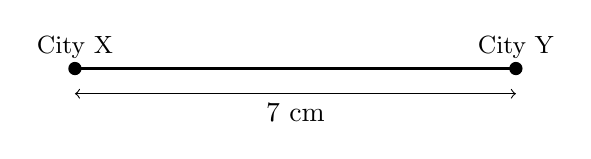
\begin{tikzpicture}[scale=0.8]
  \draw[thick] (0,0) -- (7,0);
  \fill (0,0) circle (3pt) node[above] {\small City X};
  \fill (7,0) circle (3pt) node[above] {\small City Y};
  \draw[<->] (0,-0.4) -- (7,-0.4);
  \node[below] at (3.5,-0.4) {$7$ cm};
\end{tikzpicture}
\end{center}
\end{questionText}
\correctAnswer{$280$ km}
\explanation{Multiply map distance by scale factor: $7 \times 40 = 280$ km.}
\end{practiceQuestion}

\begin{practiceQuestion}{6-1-q27}{gsa}
\begin{questionText}
A blueprint shows a square patio with a scale of $1$ in $= 3$ ft. Determine the actual perimeter of the patio.

\begin{center}
\begin{tikzpicture}[scale=0.7]
  \draw[thick,fill=funOrange!10] (0,0) rectangle (4,4);
  \draw[<->] (0,-0.4) -- (4,-0.4);
  \node[below] at (2,-0.4) {$4$ in};
  \node at (2,2) {\small Patio};
\end{tikzpicture}
\end{center}
\end{questionText}
\correctAnswer{$48$ ft}
\explanation{Actual side: $4 \times 3 = 12$ ft. Perimeter: $4 \times 12 = 48$ ft.}
\end{practiceQuestion}
